% Created by tikzDevice version 0.12.3.1 on 2023-04-01 16:37:41
% !TEX encoding = UTF-8 Unicode
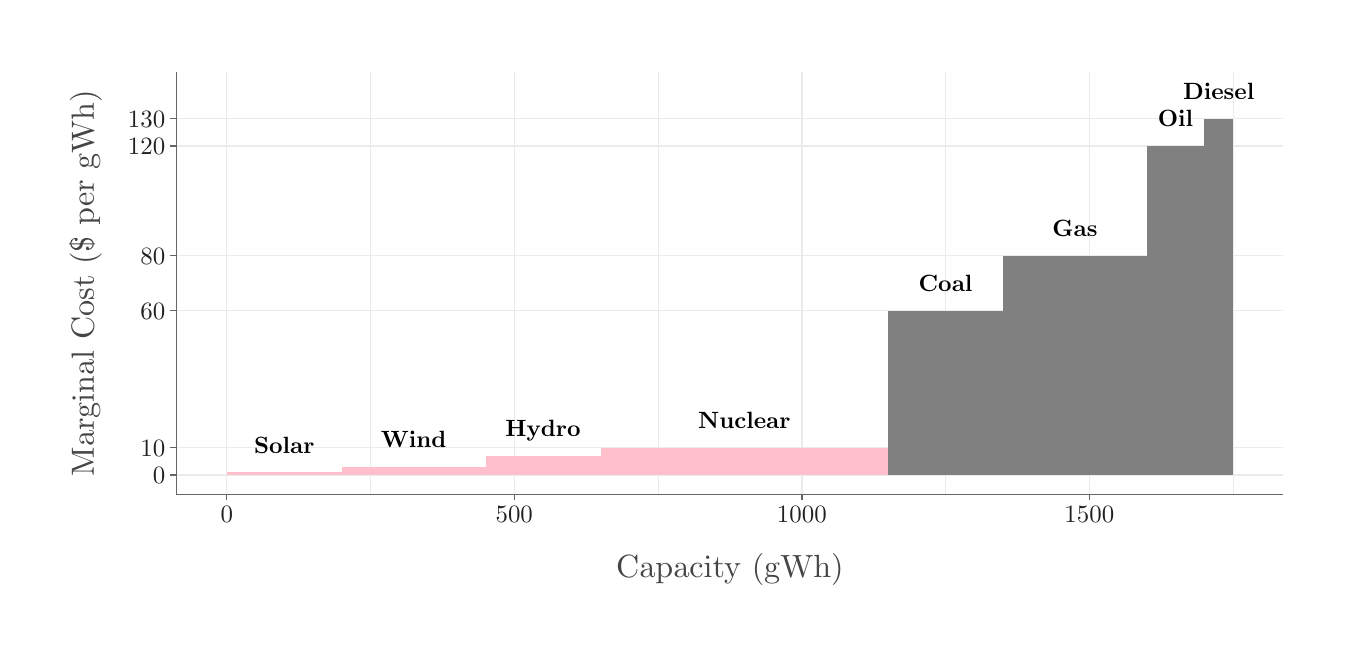
\begin{tikzpicture}[x=1pt,y=1pt]
\definecolor{fillColor}{RGB}{255,255,255}
\path[use as bounding box,fill=fillColor,fill opacity=0.00] (0,0) rectangle (469.75,216.81);
\begin{scope}
\path[clip] (  0.00,  0.00) rectangle (469.75,216.81);
\definecolor{fillColor}{RGB}{255,255,255}

\path[fill=fillColor] ( -0.00,  0.00) rectangle (469.76,216.81);
\end{scope}
\begin{scope}
\path[clip] ( 53.76, 48.21) rectangle (453.76,200.81);
\definecolor{fillColor}{RGB}{255,255,255}

\path[fill=fillColor] ( 53.76, 48.21) rectangle (453.75,200.81);
\definecolor{drawColor}{gray}{0.92}

\path[draw=drawColor,line width= 0.2pt,line join=round] (123.89, 48.21) --
	(123.89,200.81);

\path[draw=drawColor,line width= 0.2pt,line join=round] (227.78, 48.21) --
	(227.78,200.81);

\path[draw=drawColor,line width= 0.2pt,line join=round] (331.68, 48.21) --
	(331.68,200.81);

\path[draw=drawColor,line width= 0.2pt,line join=round] (435.57, 48.21) --
	(435.57,200.81);

\path[draw=drawColor,line width= 0.5pt,line join=round] ( 53.76, 55.14) --
	(453.76, 55.14);

\path[draw=drawColor,line width= 0.5pt,line join=round] ( 53.76, 65.05) --
	(453.76, 65.05);

\path[draw=drawColor,line width= 0.5pt,line join=round] ( 53.76,114.60) --
	(453.76,114.60);

\path[draw=drawColor,line width= 0.5pt,line join=round] ( 53.76,134.42) --
	(453.76,134.42);

\path[draw=drawColor,line width= 0.5pt,line join=round] ( 53.76,174.05) --
	(453.76,174.05);

\path[draw=drawColor,line width= 0.5pt,line join=round] ( 53.76,183.96) --
	(453.76,183.96);

\path[draw=drawColor,line width= 0.5pt,line join=round] ( 71.94, 48.21) --
	( 71.94,200.81);

\path[draw=drawColor,line width= 0.5pt,line join=round] (175.83, 48.21) --
	(175.83,200.81);

\path[draw=drawColor,line width= 0.5pt,line join=round] (279.73, 48.21) --
	(279.73,200.81);

\path[draw=drawColor,line width= 0.5pt,line join=round] (383.63, 48.21) --
	(383.63,200.81);
\definecolor{fillColor}{RGB}{255,192,203}

\path[fill=fillColor] ( 71.94, 55.14) rectangle (113.50, 56.13);

\path[fill=fillColor] (113.50, 55.14) rectangle (165.44, 58.12);

\path[fill=fillColor] (165.44, 55.14) rectangle (207.00, 62.08);

\path[fill=fillColor] (207.00, 55.14) rectangle (310.90, 65.05);
\definecolor{fillColor}{gray}{0.50}

\path[fill=fillColor] (310.90, 55.14) rectangle (352.46,114.60);

\path[fill=fillColor] (352.46, 55.14) rectangle (404.40,134.42);

\path[fill=fillColor] (404.40, 55.14) rectangle (425.18,174.05);

\path[fill=fillColor] (425.18, 55.14) rectangle (435.57,183.96);
\definecolor{drawColor}{RGB}{0,0,0}

\node[text=drawColor,anchor=base,inner sep=0pt, outer sep=0pt, scale=  0.85] at ( 92.72, 63.10) {\bfseries Solar};

\node[text=drawColor,anchor=base,inner sep=0pt, outer sep=0pt, scale=  0.85] at (139.47, 65.08) {\bfseries Wind};

\node[text=drawColor,anchor=base,inner sep=0pt, outer sep=0pt, scale=  0.85] at (186.22, 69.04) {\bfseries Hydro};

\node[text=drawColor,anchor=base,inner sep=0pt, outer sep=0pt, scale=  0.85] at (258.95, 72.02) {\bfseries Nuclear};

\node[text=drawColor,anchor=base,inner sep=0pt, outer sep=0pt, scale=  0.85] at (331.68,121.56) {\bfseries Coal};

\node[text=drawColor,anchor=base,inner sep=0pt, outer sep=0pt, scale=  0.85] at (378.43,141.38) {\bfseries Gas};

\node[text=drawColor,anchor=base,inner sep=0pt, outer sep=0pt, scale=  0.85] at (414.79,181.02) {\bfseries Oil};

\node[text=drawColor,anchor=base,inner sep=0pt, outer sep=0pt, scale=  0.85] at (430.38,190.93) {\bfseries Diesel};

\path[] ( 53.76, 48.21) rectangle (453.75,200.81);
\end{scope}
\begin{scope}
\path[clip] (  0.00,  0.00) rectangle (469.75,216.81);
\definecolor{drawColor}{gray}{0.40}

\path[draw=drawColor,line width= 0.5pt,line join=round] ( 53.76, 48.21) --
	( 53.76,200.81);
\end{scope}
\begin{scope}
\path[clip] (  0.00,  0.00) rectangle (469.75,216.81);
\definecolor{drawColor}{gray}{0.13}

\node[text=drawColor,anchor=base east,inner sep=0pt, outer sep=0pt, scale=  0.90] at ( 49.71, 52.04) {0};

\node[text=drawColor,anchor=base east,inner sep=0pt, outer sep=0pt, scale=  0.90] at ( 49.71, 61.95) {10};

\node[text=drawColor,anchor=base east,inner sep=0pt, outer sep=0pt, scale=  0.90] at ( 49.71,111.50) {60};

\node[text=drawColor,anchor=base east,inner sep=0pt, outer sep=0pt, scale=  0.90] at ( 49.71,131.32) {80};

\node[text=drawColor,anchor=base east,inner sep=0pt, outer sep=0pt, scale=  0.90] at ( 49.71,170.96) {120};

\node[text=drawColor,anchor=base east,inner sep=0pt, outer sep=0pt, scale=  0.90] at ( 49.71,180.86) {130};
\end{scope}
\begin{scope}
\path[clip] (  0.00,  0.00) rectangle (469.75,216.81);
\definecolor{drawColor}{gray}{0.40}

\path[draw=drawColor,line width= 0.5pt,line join=round] ( 51.51, 55.14) --
	( 53.76, 55.14);

\path[draw=drawColor,line width= 0.5pt,line join=round] ( 51.51, 65.05) --
	( 53.76, 65.05);

\path[draw=drawColor,line width= 0.5pt,line join=round] ( 51.51,114.60) --
	( 53.76,114.60);

\path[draw=drawColor,line width= 0.5pt,line join=round] ( 51.51,134.42) --
	( 53.76,134.42);

\path[draw=drawColor,line width= 0.5pt,line join=round] ( 51.51,174.05) --
	( 53.76,174.05);

\path[draw=drawColor,line width= 0.5pt,line join=round] ( 51.51,183.96) --
	( 53.76,183.96);
\end{scope}
\begin{scope}
\path[clip] (  0.00,  0.00) rectangle (469.75,216.81);
\definecolor{drawColor}{gray}{0.40}

\path[draw=drawColor,line width= 0.5pt,line join=round] ( 53.76, 48.21) --
	(453.76, 48.21);
\end{scope}
\begin{scope}
\path[clip] (  0.00,  0.00) rectangle (469.75,216.81);
\definecolor{drawColor}{gray}{0.40}

\path[draw=drawColor,line width= 0.5pt,line join=round] ( 71.94, 45.96) --
	( 71.94, 48.21);

\path[draw=drawColor,line width= 0.5pt,line join=round] (175.83, 45.96) --
	(175.83, 48.21);

\path[draw=drawColor,line width= 0.5pt,line join=round] (279.73, 45.96) --
	(279.73, 48.21);

\path[draw=drawColor,line width= 0.5pt,line join=round] (383.63, 45.96) --
	(383.63, 48.21);
\end{scope}
\begin{scope}
\path[clip] (  0.00,  0.00) rectangle (469.75,216.81);
\definecolor{drawColor}{gray}{0.13}

\node[text=drawColor,anchor=base,inner sep=0pt, outer sep=0pt, scale=  0.90] at ( 71.94, 37.96) {0};

\node[text=drawColor,anchor=base,inner sep=0pt, outer sep=0pt, scale=  0.90] at (175.83, 37.96) {500};

\node[text=drawColor,anchor=base,inner sep=0pt, outer sep=0pt, scale=  0.90] at (279.73, 37.96) {1000};

\node[text=drawColor,anchor=base,inner sep=0pt, outer sep=0pt, scale=  0.90] at (383.63, 37.96) {1500};
\end{scope}
\begin{scope}
\path[clip] (  0.00,  0.00) rectangle (469.75,216.81);
\definecolor{drawColor}{gray}{0.27}

\node[text=drawColor,anchor=base,inner sep=0pt, outer sep=0pt, scale=  1.16] at (253.76, 18.25) {Capacity (gWh)};
\end{scope}
\begin{scope}
\path[clip] (  0.00,  0.00) rectangle (469.75,216.81);
\definecolor{drawColor}{gray}{0.27}

\node[text=drawColor,rotate= 90.00,anchor=base,inner sep=0pt, outer sep=0pt, scale=  1.16] at ( 23.96,124.51) {Marginal Cost (\$ per gWh)};
\end{scope}
\end{tikzpicture}
